\chapter{Modré karty}
Poradie ťahania na začiatku ťahu je: Dynamit $\rightarrow$ Väzenie $\rightarrow$ Chřestýš. Hráč zároveň nemôže mať pred sebou vyložené dve karty s rovnakým názvom.
\begin{comment}
\begin{figure}[!h]
\begin{minipage}[t]{\minipageSize}\centering
  \includegraphics[width=\cardSize\linewidth]{}
 \caption[]{}
  \label{fig:bang}
\end{minipage}
\hfill
\begin{minipage}[t]{\minipageSize}\centering
  \includegraphics[width=\cardSize\linewidth]{}
  \caption[]{}
  \label{fig:vedle}
\end{minipage}
\hfill
\begin{minipage}[t]{\minipageSize}\centering
  \includegraphics[width=\cardSize\linewidth]{}
  \caption[]{}
  \label{fig:duel}
\end{minipage}
\hfill
\begin{minipage}[t]{\minipageSize}\centering
  \includegraphics[width=\cardSize\linewidth]{}
\caption[]{}
  \label{fig:panico}
\end{minipage}
\end{figure}
\end{comment}

\begin{figure}[!h]
\begin{minipage}[t]{\minipageSize}\centering
  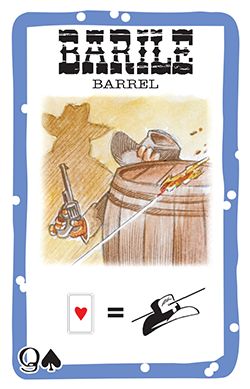
\includegraphics[width=\cardSize\linewidth]{Modre karty/01_barile.png}
 \caption[Barel]{Ak je hráč cieľom efektu Bang! alebo inej karty so symbolom Bang!, môže ťahať vrchnú kartu balíčka. Ak je srdcová, získa efekt Vedle!. Na jeden prichádzajúci útok sa na Barel ťahá najviac raz, ak pravidlo výslovne nehovorí inak.}
  \label{fig:bang}
\end{minipage}
\hfill
\begin{minipage}[t]{\minipageSize}\centering
  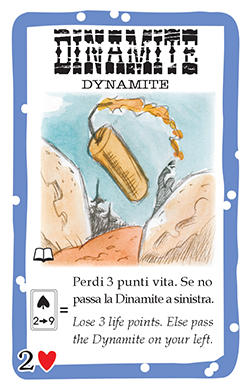
\includegraphics[width=\cardSize\linewidth]{Modre karty/01_dinamite.png}
  \caption[Dynamit]{Ak je karta pred hráčom, pred fázou 1 si musí z baláčka ťahať kartu. Pokiaľ je karta listová s hodnotou 2 až 9, dynamit vybuchne, hráč stráca 3 životy a karta sa odhodí. V opačnom prípade sa posúva hráčovi po jeho ľavici. Hráč nemôže mať pred sebou 2 dynamity. Ak by sa mu mal posunúť druhý dynamit tak ho posúva automaticky ďalej.}
  \label{fig:vedle}
\end{minipage}
\hfill
\begin{minipage}[t]{\minipageSize}\centering
  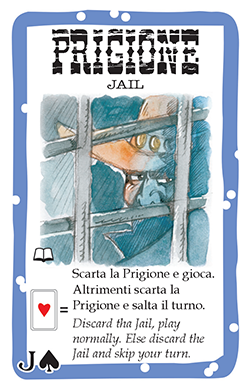
\includegraphics[width=\cardSize\linewidth]{Modre karty/01_prigione.png}
  \caption[Vězení]{Pred fázou 1 si hráč musí ťahať kartu z balíčku. Pokiaľ je srdcová, môže začať svoj ťah a väzenie sa odhodí. V opačnom pípade vynecháva ťah (aj chřestýša a ťahanie na iné karty) a karta sa odhadzuje.}
  \label{fig:duel}
\end{minipage}
\hfill
\begin{minipage}[t]{\minipageSize}\centering
  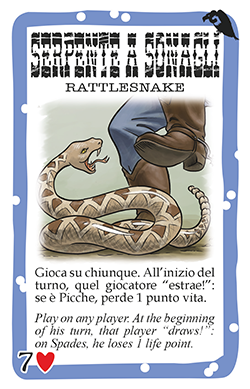
\includegraphics[width=\cardSize\linewidth]{Modre karty/07_serpenteasonagli.png}
\caption[Chřestýš]{Pred fázou 1 si musí hráč ťahať kartu z balíčka. Pokiaľ je listová, stráca hráč 1 život. Chřestýš ostáva pred hráčom aj po spôsobení zranenia a odstráni sa len iným efektom, napr. Panikou alebo Cat Balou. Poradie kontrol na začiatku ťahu je: Dynamit, potom Väzenie, potom Chřestýš.}
  \label{fig:panico}
\end{minipage}
\end{figure}

\begin{figure}[!h]
\begin{minipage}[t]{\minipageSize}\centering
  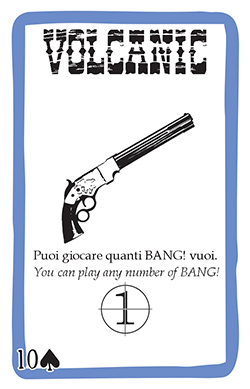
\includegraphics[width=\cardSize\linewidth]{Modre karty/01_volcanic.png}
 \caption[Volcanic]{Hráč môže za svoj ťah použiť ľubovoľný počet kariet Bang! na dosah 1. Dosah môžu zvýšiť karty vyložené pred hráčom.}
  \label{fig:bang}
\end{minipage}
\hfill
\begin{minipage}[t]{\minipageSize}\centering
  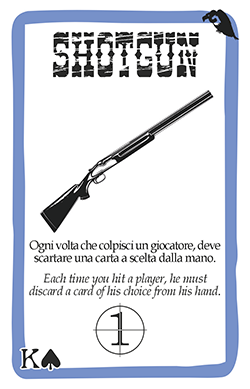
\includegraphics[width=\cardSize\linewidth]{Modre karty/07_shotgun.png}
  \caption[Brokovnice]{Hráč, ktorý je zasiahnutý kartou Bang! z tejto zbrane musí odhodiť kartu z ruky podľa svojho výberu. Dosah 1. Keď má hráč poslený život a má na ruke jedinú kartu, a to Pivo, odovzdáva Pivo hráćovi ktorý ho zasiahol a je vyradený z hry. }
  \label{fig:vedle}
\end{minipage}
\hfill
\begin{minipage}[t]{\minipageSize}\centering
  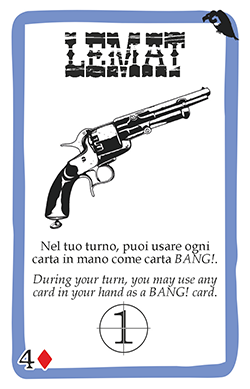
\includegraphics[width=\cardSize\linewidth]{Modre karty/07_lemat.png}
  \caption[Lemat]{Hráč môže použiť ľubovoľnú kartu z ruky ako kartu Bang!, okrem karty Vedle!. Dosah je 1. Takto zahraná karta sa počíta do limitu Bang!.}
  \label{fig:duel}
\end{minipage}
\hfill
\begin{minipage}[t]{\minipageSize}\centering
  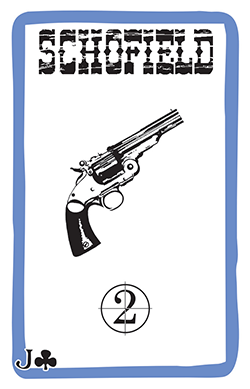
\includegraphics[width=\cardSize\linewidth]{Modre karty/01_schofield.png}
\caption[Achofield]{Zvýšenie dosahu na 2.}
  \label{fig:panico}
\end{minipage}
\end{figure}

\begin{figure}[!h]
\begin{minipage}[t]{\minipageSize}\centering
  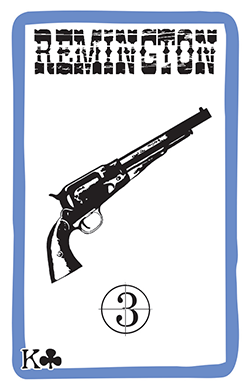
\includegraphics[width=\cardSize\linewidth]{Modre karty/01_remington.png}
 \caption[Remington]{Zvýšenie dosahu na 3.}
  \label{fig:bang}
\end{minipage}
\hfill
\begin{minipage}[t]{\minipageSize}\centering
  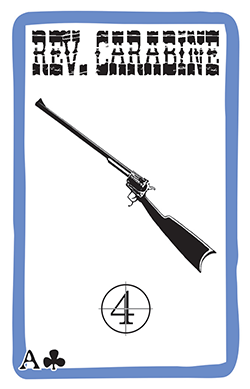
\includegraphics[width=\cardSize\linewidth]{Modre karty/01_carabine.png}
  \caption[Rev. Carabine]{Zvýšenie dosahu na 4.}
  \label{fig:vedle}
\end{minipage}
\hfill
\begin{minipage}[t]{\minipageSize}\centering
  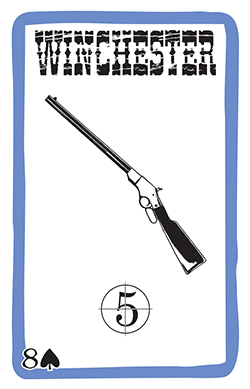
\includegraphics[width=\cardSize\linewidth]{Modre karty/01_winchester.png}
  \caption[Winchester]{Zvýšenie dosahu na 5.}
  \label{fig:duel}
\end{minipage}
\hfill
\begin{minipage}[t]{\minipageSize}\centering
  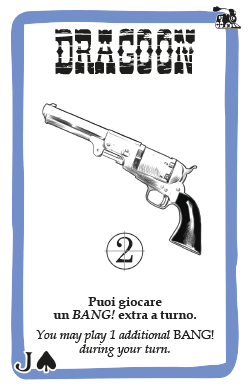
\includegraphics[width=\cardSize\linewidth]{Modre karty/27_Dragoon.png}
  \caption[Dragoon]{Hráč môže vo svojom ťahu zahrať o jednu kartu Bang! navyše na vzdialenosť 2.}
  \label{fig:vedle}
\end{minipage}
\end{figure}

\begin{figure}[!h]
\begin{minipage}[t]{\minipageSize}\centering
  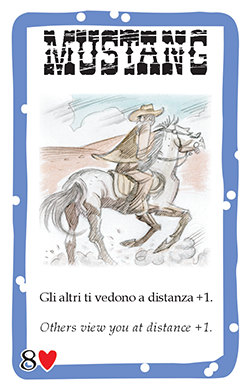
\includegraphics[width=\cardSize\linewidth]{Modre karty/01_mustang.png}
 \caption[Mustang]{Vzdialenosť od všetkých hráčov (z ich prespektívy) je väčšia o 1.}
  \label{fig:bang}
\end{minipage}
\hfill
\begin{minipage}[t]{0.22\linewidth}\centering
  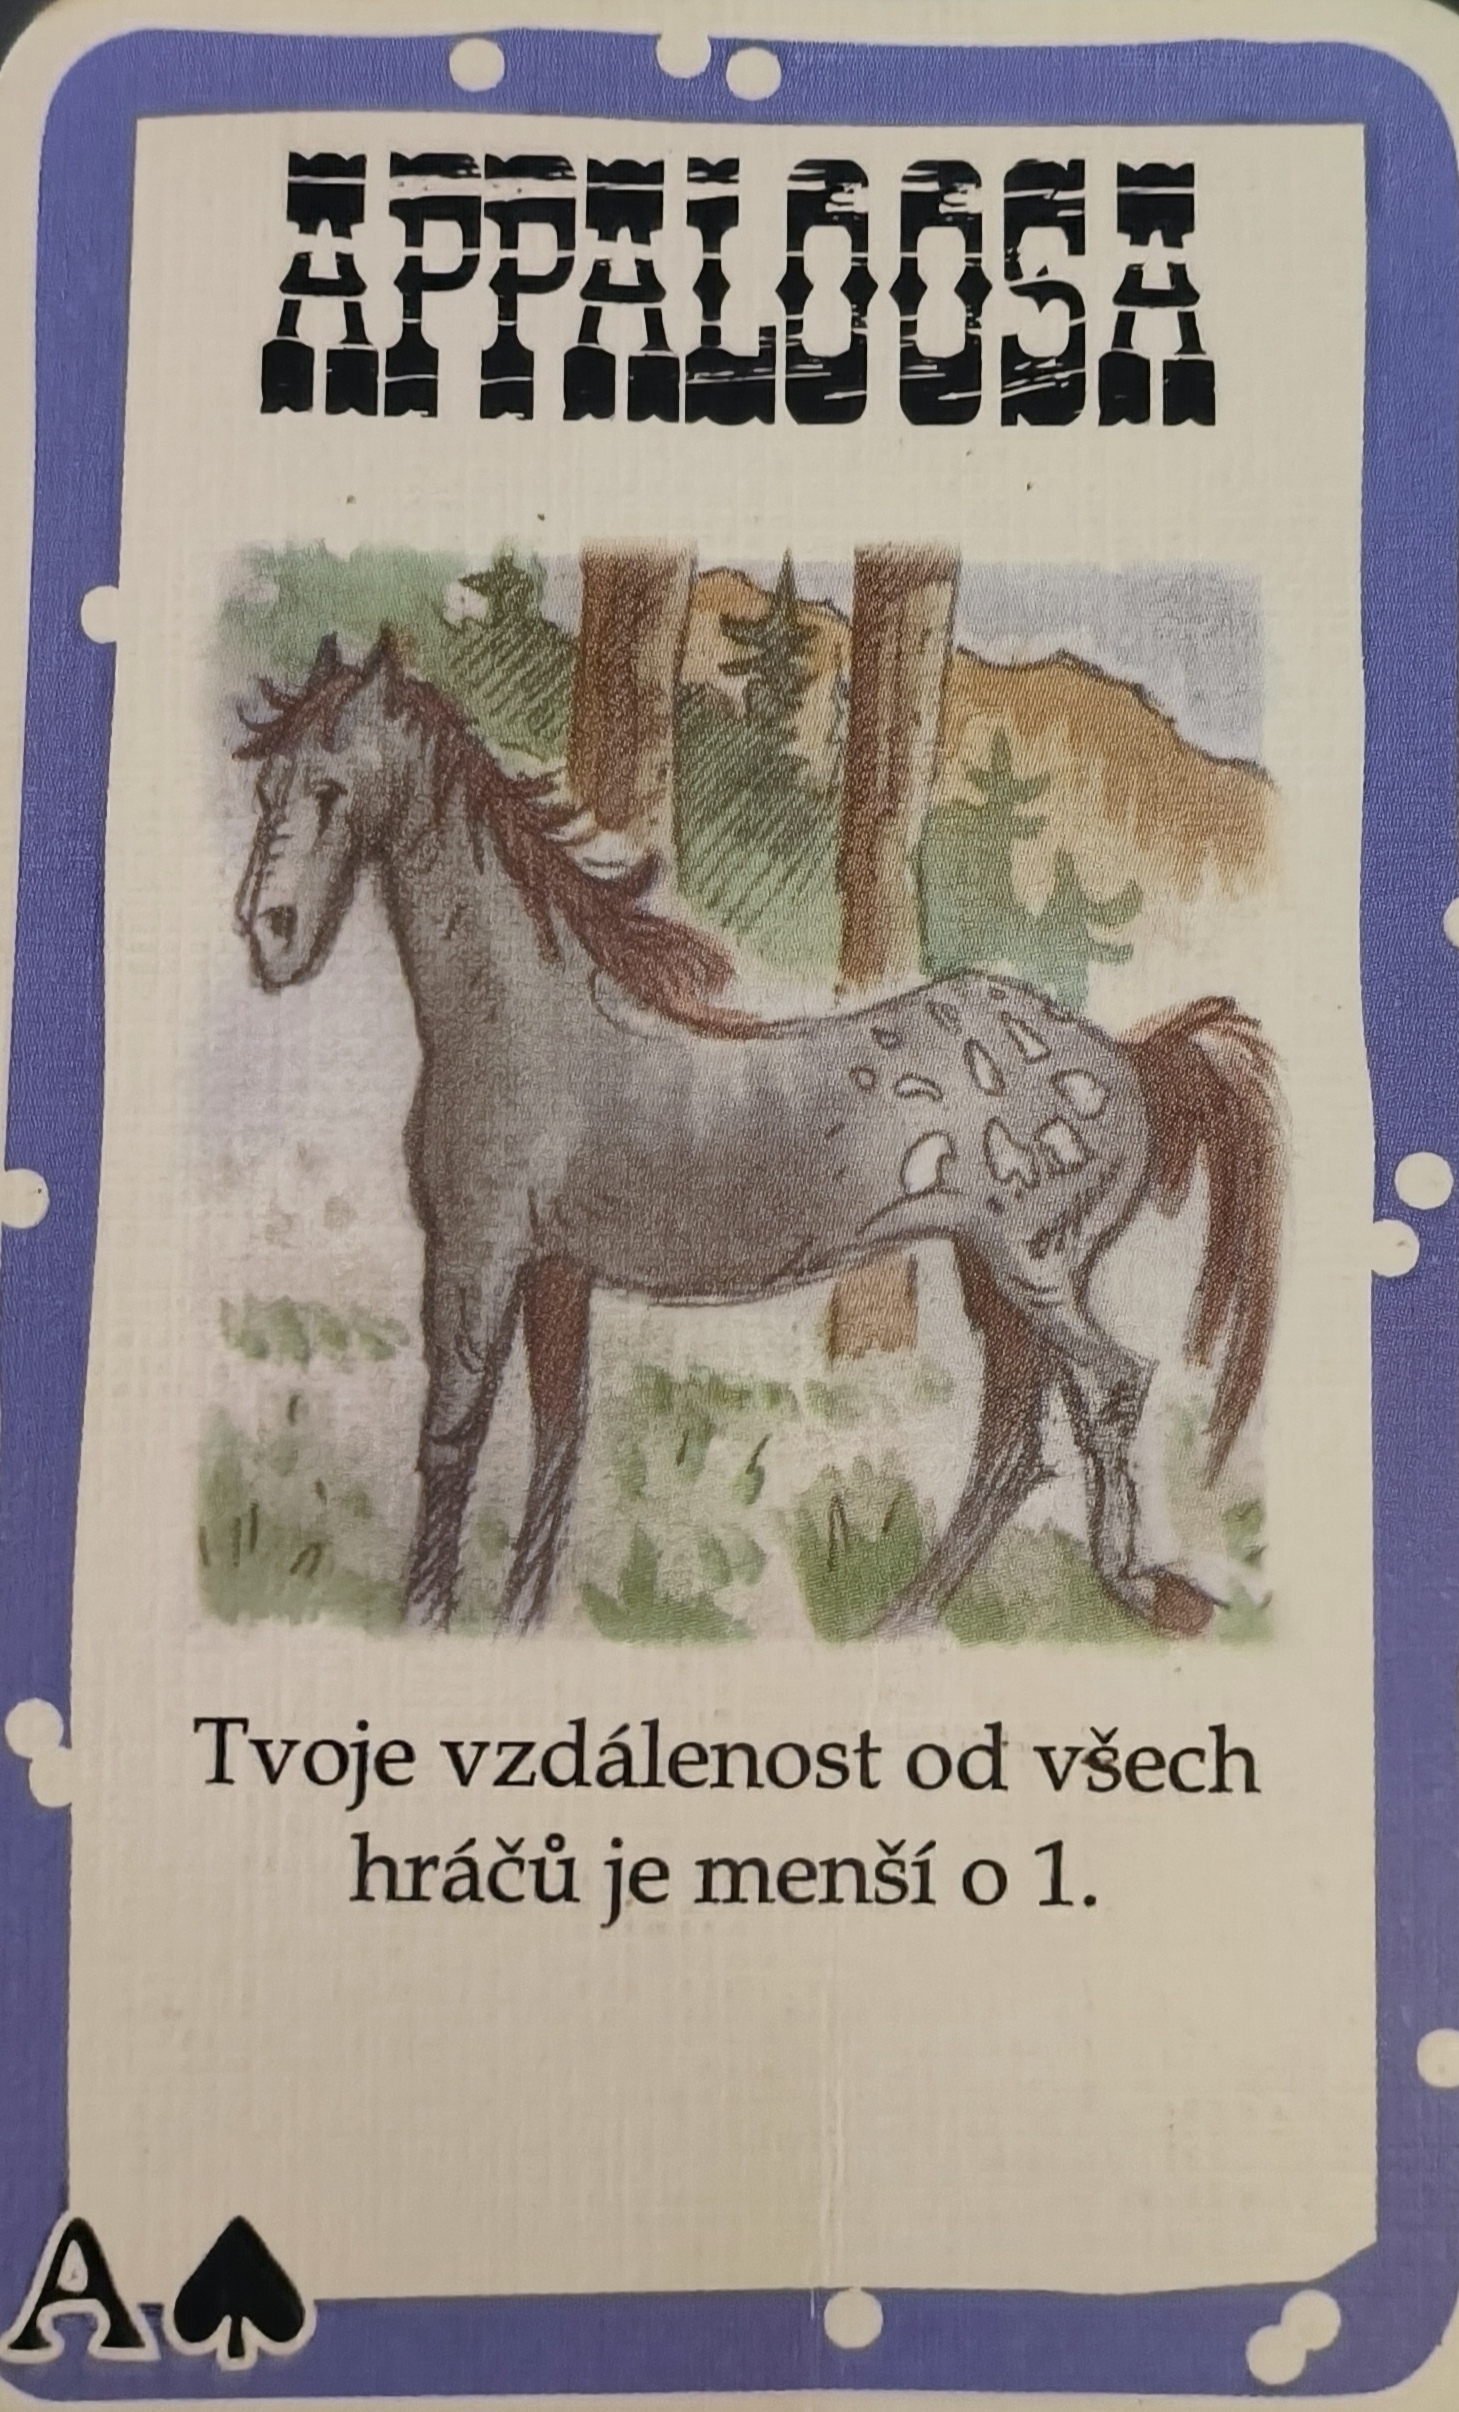
\includegraphics[width=\cardSize\linewidth]{Modre karty/Appaloosa.jpg}
  \caption[Appaloosa]{Vzdiaľenosť od všetkých hráčov (z vašej perspektívy) je menšia o 1.}
  \label{fig:vedle}
\end{minipage}
\hfill
\begin{minipage}[t]{0.225\linewidth}\centering
  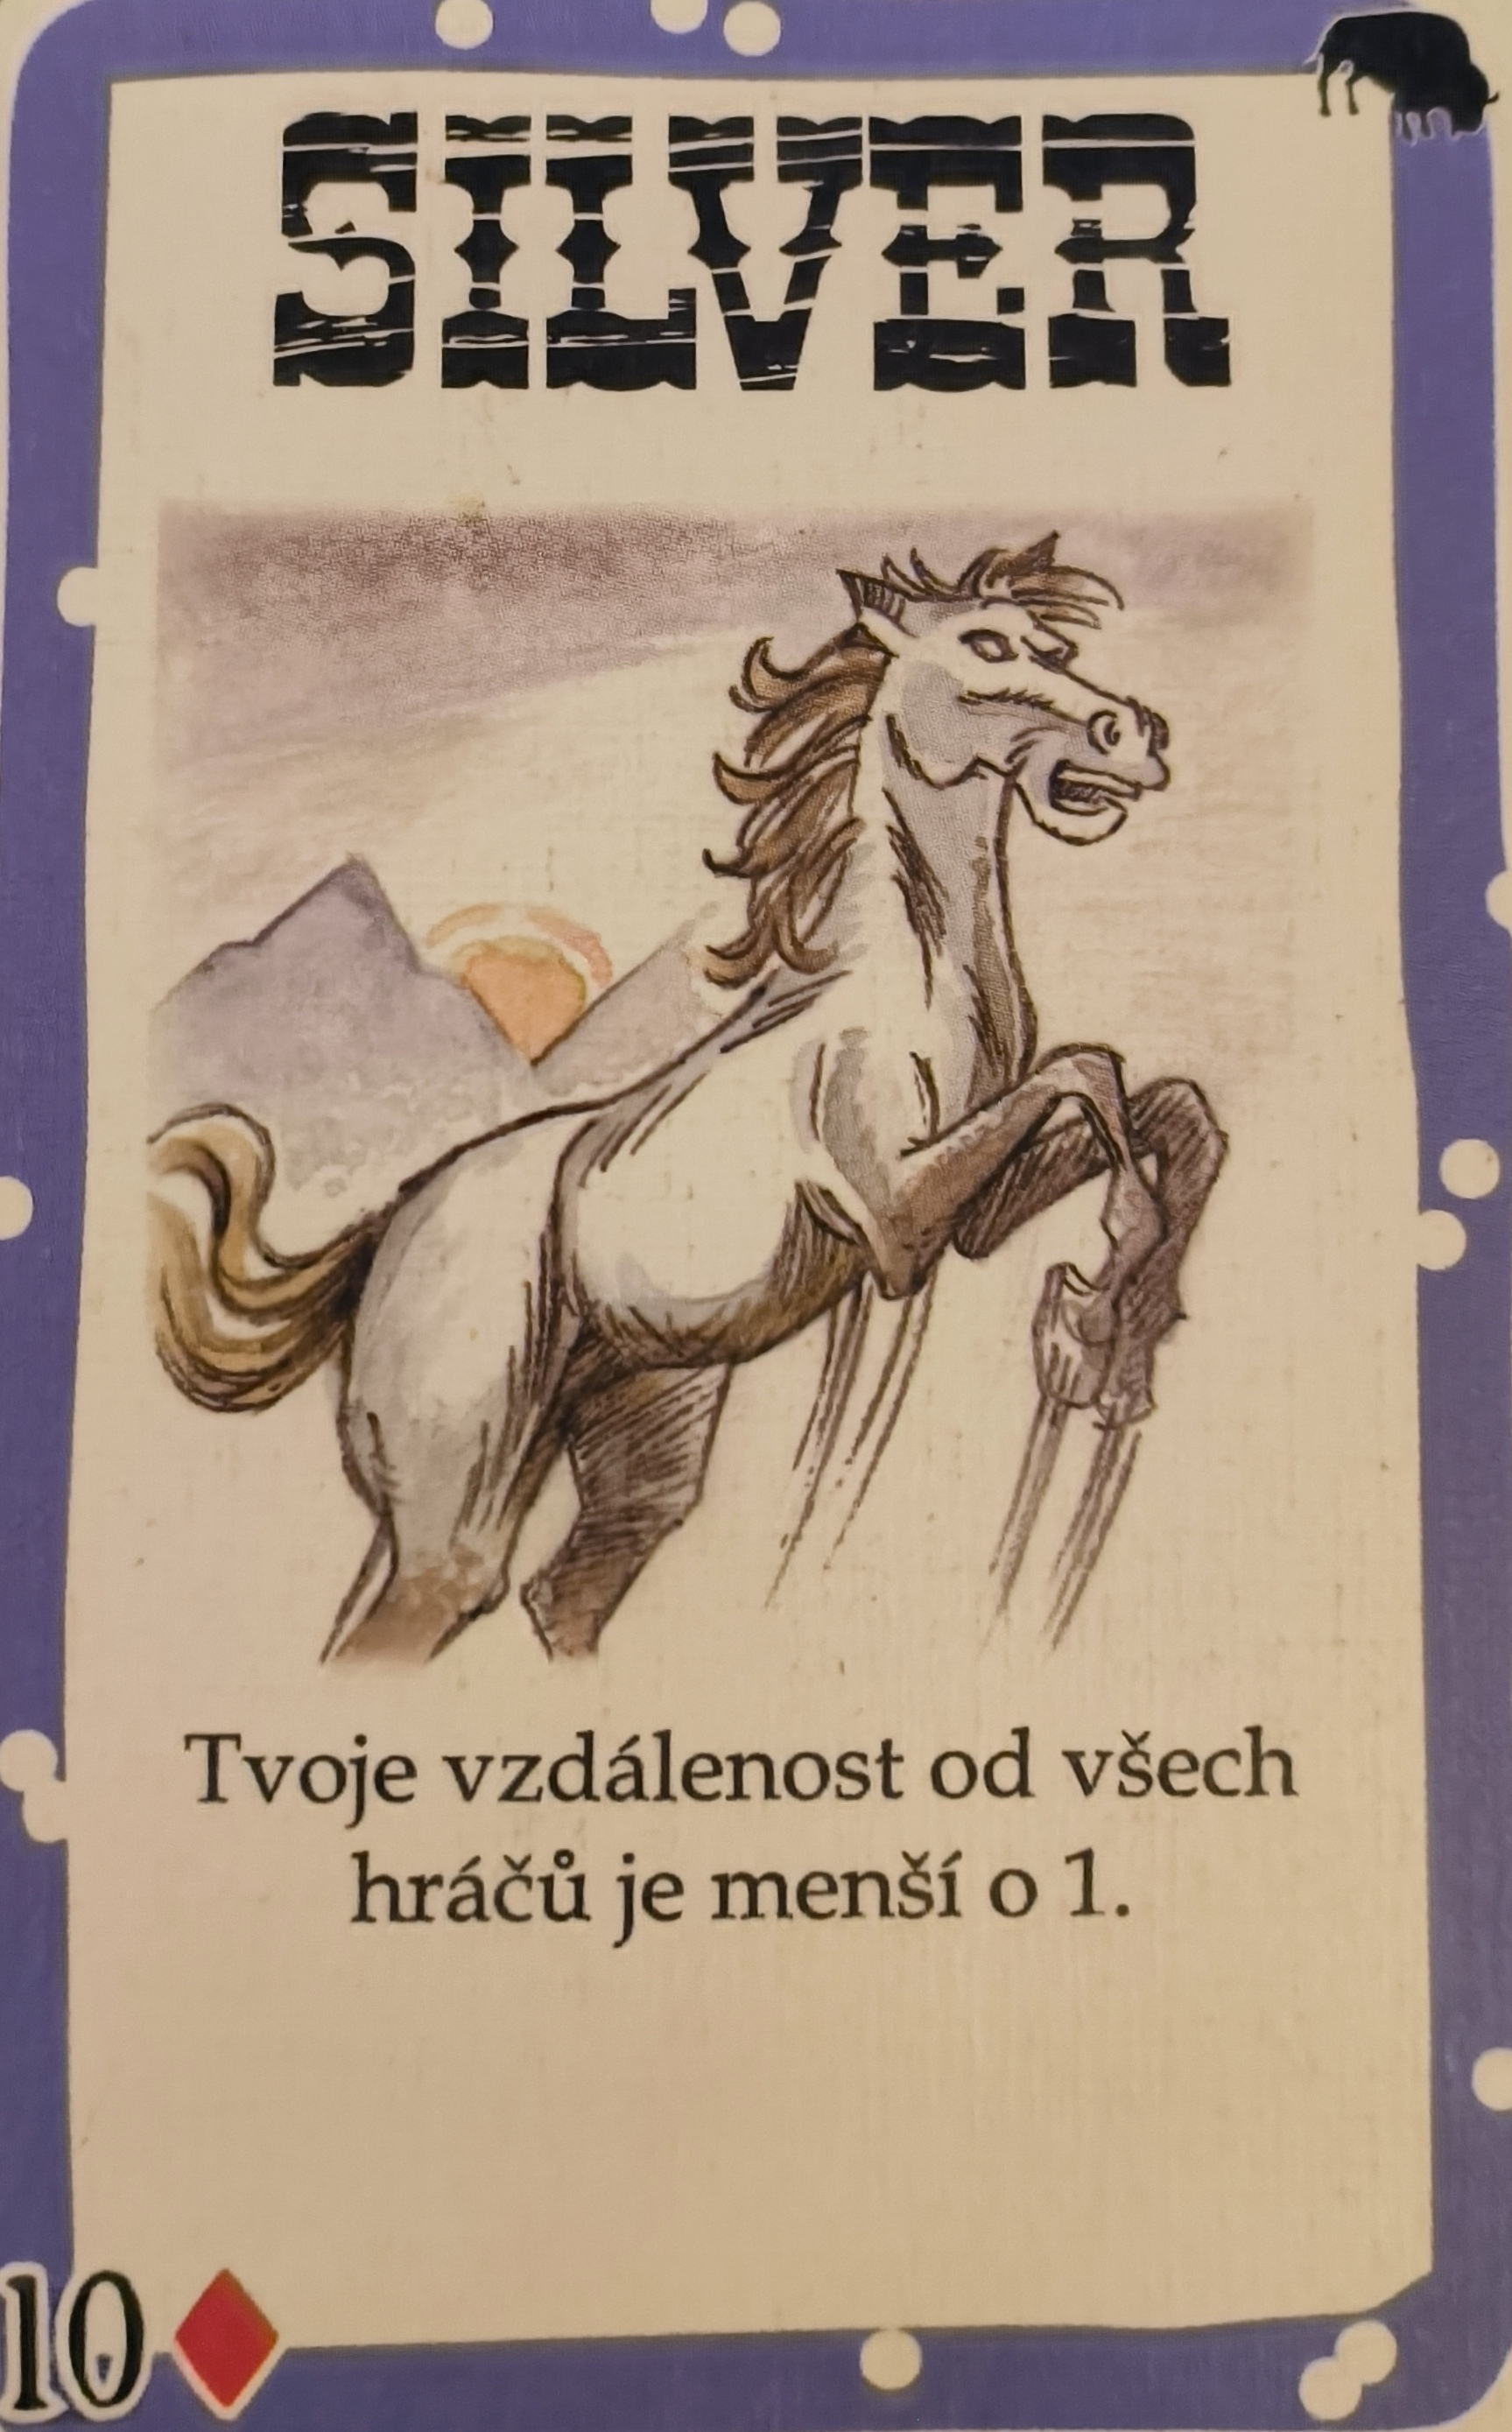
\includegraphics[width=\cardSize\linewidth]{Modre karty/Silver.jpg}
  \caption[Silver]{Vzdiaľenosť od všetkých hráčov (z vašej perspektívy) je menšia o 1.}
  \label{fig:duel}
\end{minipage}
\hfill
\begin{minipage}[t]{\minipageSize}\centering
  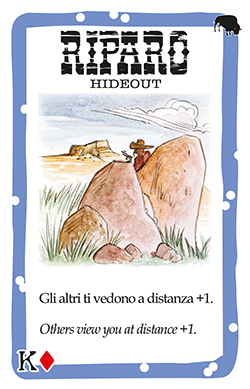
\includegraphics[width=\cardSize\linewidth]{Modre karty/03_riparo.png}
\caption[Skrýš]{Vzdialenosť od všetkých hráčov (z ich prespektívy) je väčšia o 1.}
  \label{fig:panico}
\end{minipage}
\end{figure}

\begin{figure}[!h]
\begin{minipage}[t]{\minipageSize}\centering
  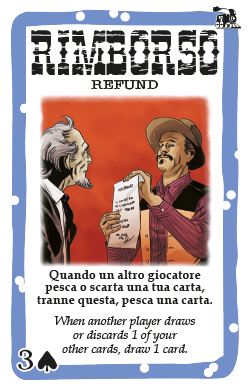
\includegraphics[width=\cardSize\linewidth]{Modre karty/30_Refund.png}
 \caption[Odškodnění]{Pokiaľ niektorý hráč odoberie alebo odhodí kartu z ruky alebo z hry inému hráčovi, ťahá si poškodený hráč kartu z balíčku. Nefunguje proti vlakovej loupeži. }
  \label{fig:bang}
\end{minipage}
\hfill
\begin{minipage}[t]{\minipageSize}\centering
  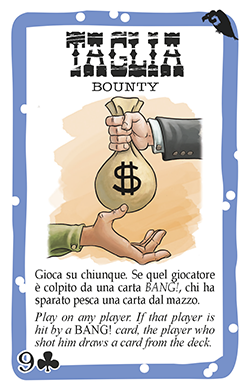
\includegraphics[width=\cardSize\linewidth]{Modre karty/07_taglia.png}
\caption[Odměna]{Pokladá sa pred ľubovoľného hráča. Pokiaľ je hráč zasiahnutý kartou Bang!, hráč ktorý ho zasiahol si potiahne kartu z balíčka.}
  \label{fig:panico}
\end{minipage}
\hfill
\begin{minipage}[t]{\minipageSize}\centering
  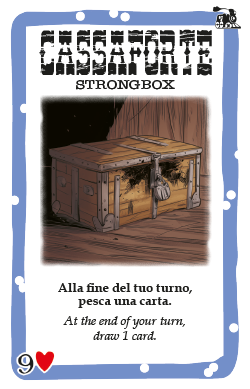
\includegraphics[width=\cardSize\linewidth]{Modre karty/28_Strongbox.png}
  \caption[Pokladnica]{Na konci svojho ťahu si hráč potiahne 1 kartu z balíčka. Platí to aj vtedy, keď sa v danom kole nedostal z Väzenia. Takto potiahnutú kartu už v tom istom ťahu nemožno zahrať.}
  \label{fig:duel}
\end{minipage}
\hfill
\begin{minipage}[t]{\minipageSize}\centering
  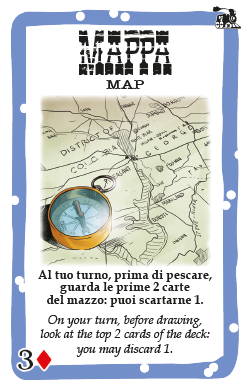
\includegraphics[width=\cardSize\linewidth]{Modre karty/29_Map.png}
\caption[Mapa]{Predtým, než si vo fáze 1 potiahnete karty, pozrite sa na 2 vrchné karty balíčka, jednu z nich odhoďte a druhú vráťte naspäť na vrch. Tento efekt sa vyhodnocuje po všetkých ťahoch na Dynamit, Väzenie a podobné karty, ale ešte pred schopnosťami postáv.}
  \label{fig:panico}
\end{minipage}
\end{figure}

\begin{figure}[!h]
\centering
\begin{minipage}[t]{\minipageSize}
  \centering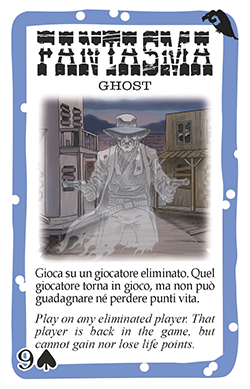
\includegraphics[width=\cardSize\linewidth]{Modre karty/07_fantasma.png}
 \caption[Duch]{Karta sa pokladá pred ľubovoľného vyradeného hráča. Hráč sa tým pádom vracia do hry bez schopností a bez životov. 
 Hrá ako normálny hráč, teda môže pred seba vykladať karty, tvorí vzdialenosť, ťahá na hokynářství, môže byť poslaný do Väzenia, ťahá si na Dynamit atď.
Na konci svojho ťahu musí odhodiť všetky karty z ruky, keďže má 0 životov. Ak je karta Duch odstránená, tento hráč okamžite znova opúšťa hru. 
Pokiaľ má hráč Ducha, Mŕtvy muž naňho neplatí aj keď hráč umrel ako prvý. \\
Pr. 1: Šerif je živý, odpadlík má ducha a nikto iný nie je v hre. Hra pokračuje pokiaľ odpadlík nezabije šerifa alebo šerif neodstrání ducha z pred odpadlíka. \\
Pr. 2: Šerif a odpadlík sú živí, Vice má ducha a odpadlík zabije šerifa, vyhrávajú banditi, lebo Vice je stále v hre.\\ 
Pr. 3: Je v hre Belle Star a je na svojom ťahu. Efekt karty duch sa vtedy eliminuje. Čiže ak je Belle Star odpadlík, je zabitý šerif a ducha má vice, vyhráva Belle Star ako odpadlík.}
  \label{fig:bang}
\end{minipage}

\vfill
\end{figure}
